% -----------------------------------------------------------------------------
% 1) Paint a story line of developments beginning from SIR
% 2) Give adequate breakdown of types of models:
%.   -  Percolation-based lattice models 
%    -  Non-local dispersal models culminating in the meta-population model
%    -  The continuum-based PDE models ? Spatial SIR models
%.   -  Network models ? 
% 3) Give a breakdown of control methods with these types of models
%.   - Clear examples of how mathematical and computational models inform policy
% -----------------------------------------------------------------------------


\chapter{Modelling infectious tree diseases}
\label{chapter2:litreview} 

The mathematical and computational modelling of infectious tree diseases began to emerge after Plank had others put forward seminal works on the modelling of crops. Tree disease is import to consider for tree-health in both commercially cultured of stands and naturally occurring forestry and ecosystems. The modelling tree-based disease has many features in common with modelling crop diseases. However, differences in the spatial distribution of hosts and growth cycles remain large.\\

The aim of tree disease modelling is to help design effective control policies. From well designed control policies, the spread of disease through commercial and rural environments can be managed and tree-health maintained. This chapter begins with a chronological overview of tree disease models and the different approaches that have been used in the past.\\

Having reviewed typical models in literature, the theme of control will be reviewed. That is, how the optimal control of a pathogen can be investigated from the construction of models.\\

Modern Epidemiology is extremely interdisciplinary utilising various tools from mathematics, physics and computer science. The project will explore infectious diseases specific to tree species. There have been various models used to model tree disease including: 1) Lattice-based percolation. 2) Continuum. 3) Meta-population. 4) Network models. A summary of these models will be given in this chapter along with their main usage, control. A review of epidemic control in plant populations will be given in support of chapter where we detail a novel method stop the spread of disease. 


\section{Determinism and stochasticity}

The spread of disease inherently takes the form of a stochastic process, whereby an epidemic unexpectedly arises and quickly cease, seemingly out of the blue. In order to capture the spread of disease, stochastic effects cannot be overlooked... 

\textcolor{red}{
\begin{itemize}
    \item Explain differences in modelling approaches
    \item Why use stochastic methods
    \item How do you collect results of a stochastic model ? Ensemble averaging
    \item Give an overview of some results in the literature
\end{itemize}}


\section{Dispersal}

One of the key features that distinguish tree disease from human-based disease is dispersal. The dispersal of a pathogen may take many forms..l
\textcolor{red}{
\begin{itemize}
    \item The importance of dispersal
    \item How is dispersal treated mathematically ?
    \item What type of dispersal kernels have been studied?
    \item What parameter-values have been inferred ?
    \item How long-range can dispersal be ? Talk about long-range inter-Continental dispersal
\end{itemize}}

\section{Compartmentalised models}
\label{ch2:lit-rev-compartmentalised-models}
Compartmentalised models are the dominate theme in epidemiological modelling...

% - describe how plank model can be represented in terms of a compartmentalised model \cite{time-varying-infectivity}
% In his seminal work, van der Plank \cite{van2013plant} considered a latency and infectious period, with a constant rate of infection while infectious; this model is represented by the equation:
% \begin{equation}
% \label{eq:plank-model}
%     \frac{dI(t)}{dt} = R\big(I(t - p)  - I(t - p - i)\big)\big(1 - I(t)\big)
% \end{equation}

% where $p$ and $i$ are constant latency and infectivity periods and $R$ is the corrected infection rate (i.e. including host demography). Equation \ref{eq:plank-model} is seldom used in contemporary literature, owing to the difficulty in analytically solving its time-delay \cite{madden2006botanical}. However, it provides a simple basis to understand time-varying infectivities. 

% Later, \cite{time-varying-infectivity} demonstrated that sporulation can be decomposed into a suite of $SEIR$-like models. Specifically, the authors of \cite{time-varying-infectivity} demonstrated that both compartmentalised $SEIR$ models and the plank formulation can be decomposed into a $SEmInR$ model i.e. where transitions follow $S\rightarrow E_1, E_2,.., E_m \rightarrow I_1, I_2, ..., I_n \rightarrow R$.
% By taking suitable limits of $n$ and $m$ the plank and $SEIR$ models can be recovered. 

\subsection{Lattice-based modelling}
Lattice-based models have been used to describe the spread of disease in many contexts, such as the spread of malaria, the bubonic plague and the spread of tree disease...

\textcolor{red}{
\begin{itemize}
    \item Spatial SIR model
    \item Agent-based modelling
    \item A good place to talk about Percolation models
    \item \textcolor{red}{Murray}: travelling waves that do not change shape
\end{itemize}}

\section{The role of scale}

The role of scale is crucial to describing the spread of tree-based disease...
\textcolor{red}{
\begin{itemize}
    \item The spatial aggregation of vegetation, how does clustering look on different spatial resolutions ?
    \item Spatial scale in dispersal ? What does this mean for disease gradients ?
    \item \cite{https://doi.org/10.1111/jbi.13642}
    \item \cite{ pautasso2013european}, search for 'modelling' in this review paper. It contains references to LDD models.
\end{itemize}}

\section{Modelling landscape-level epidemics}

Modernity has witnessed the spread of tree-based epidemics at the regional, country and continental level. 'landscape-level'...

\subsection{The Metapopulation model}
\begin{itemize}
    \item this variation in epidemic outcome from variants of environmental factors was likened to the metapopulation used in ecology and population dynamics in order to describe environment `patchiness'
    \item variability in the host landscape was considered and recognised as important, the patchiness of a landscape lends itself well to a metapopulation model
    \cite{doi:10.1098/rstb.1986.0072}
    \item \cite{large-scale-control}
\end{itemize}

\subsection{Network Modelling}

Network models are useful to describe the spread disease of human-based trade and transport of infectious trees...

\textcolor{red}{
\begin{itemize}
    \item What paradigm do network models suit?
    \item Human trade and transport and networks 
    \item plant-to-plant interactions and networks ? 
    \item give examples of how network models have been used in the literature
    \item review \cite{doi:10.1098/rsif.2005.0051}
\end{itemize}}

% Consider doing a chapter on `thresholds` that can incorporate Invasion & Persistence
\section{Thresholds in plant-based disease}

A key theme in the spread of tree-disease, and disease in the broadest sense, can be understood through a threshold...

\textcolor{red}{
\begin{itemize}
    \item What was the first paper to use this term ? Give mini-historical recount
    \item What is Invasion and persistence ? Give examples of papers and results in literature 
    \item The importance of thresholds
    \item Where does this number come from and why is \textbf{}this an important number ?
    \item How can one define $R_0$ ? Talk about how the there are different ways to calculate it e.g. next-generation operator 
    \item Survey what results have been obtained in the literature using $R_0$
\end{itemize}}

\subsection{The basic reproduction number}
The basic reproduction number, denoted by $R_0$, can be seen to arise in the study of population dynamics and demographics to categorize offspring \cite{heesterbeek2002brief}. In the study of epidemics, $R_0$ was adapted in order to categorize the number of infectious offspring and is widely agreed to be the most important and informative parameter. The basic reproduction number can be derived from the $SIR$ model \cite{kermack-model}, and from it, we can see how a likely disease is to spread though a population. Numerous definitions of $R_0$, and methods of determination, have been proposed in the literature resulting in confusion and multiple $R_0$ values for one pathogen \cite{delamater2019complexity}. However, a common definition states:

\textit{The expected number of secondary infections that result from one infected individual, over it's entire infectious lifetime, in a completely susceptible population.}

here, the infectious life-time is the total amount of time an individual remains infectious. The individuals infectious status will culminate in either recovery or death. Importantly, from $R_0$ a threshold can be determined which dictates whether or not the disease will spread through large parts of the population. That is, if $R_0>1$ an \textit{epidemic} will result, otherwise the spread of disease will likely halt. The value of $R_0$ can be determined from different methods\footnote{Common approaches include, the survival function, next-generation operator and estimation from epidemiological data \cite{perspectives-on-r0}} and from it many surrogate parameters can be calculated which leads to confusion \cite{diekmann2010construction}.\\

The basic reproduction number is used extensively by researchers wishing to understand the spread of disease through human populations. In the study of plant-based disease however, the basic reproduction number has attracted far less attention despite being a convenient parameter from which a threshold can be derived. Thresholds are of great importance to understand epidemics in plant-based populations. A threshold criteria similar to the $R_0$-threshold was first introduced by \cite{van2013plant} in the logistic growth model. However, the logistic-growth based threshold was a vast simplification and had limitations in accurately predicting the threshold for growth and spread \cite{onstad1992evaluation}.\\

The basic reproduction number $R_0$ was studied by \cite{gubbins2000population} in order to understand thresholds in plant-parasite \textit{pathosystems}. A plant-host under attack from a parasite may respond to the \textit{parasite load} with either the promotion or inhibition of susceptible tissue, see \cite{gilligan1997analysis} for further details on this mechanism. In order to model this problem, \cite{gubbins2000population} used a system of three linked differential equations describing the density of susceptible hosts, infected hosts and the primary source of innoculum\footnote{\textemdash here, innoculum is a general term that refers to any part of the parasite that, when in contact with the plant, may induce disease \cite{agrios2005chapter}}. Transmission of innoculum could occur through a dual source, that is, through primary or secondary pathways. Local stability analysis on the linked equations lead to various $R_0$ values, and subsequently threshold criteria, dependant on the functional form assumed by the host-response.\\

\subsection{Invasion and Persistence}
\label{ch3:invasions_and_persistence}
When calculating thresholds, the spatial structure of the host population cannot be overlooked. A study conducted by \cite{park2001invasion} considered how spatial heterogeneity effects the dynamics of plant-parasite interactions and derived the basic reproduction number for a spatially structured host population. The density of susceptible and infected hosts were comparatively examined with deterministic and stochastic model variants. The host population in \cite{park2001invasion} consisted of \textit{patches}, which in reality could be either a single host, field or region of land. Inside each patch, the \textit{within-patch} dynamics were governed by a basic reproduction number, $R_p$. If $R_p > 1$ the parasite could survive and reproduce locally or otherwise die. The infection could jump between different patches via a longer-range interaction, set by a coupling strength. Patches were locally coupled together in a neighbourhood and the infection could jump between neighboring patches. The strength of interactions between neighboring patches were set by a coupling strength $\epsilon$ which was independently of distance.\\

From the model put forward by \cite{park2001invasion}, the concept of \textit{persistence} could be observed. Persistence occurs when a pathogen can reproduce, and thus spread from host-to-host, however the the spread is slow enough such that host-regrowth can keep continually supplying the pathogen with susceptible matter. Whereas, if the pathogen spread more aggressively through the population, the supply of susceptible material would be quickly exhausted and the pathogen would quickly die.\\


% $R_0$ is a complex function which changes in time, to this end, the next generation operator is used to derive a value for $R_0$ \cite{doi:10.1098/rsif.2009.0386}.
% ref 2 \cite{doi:10.1146/annurev.phyto.011108.135838} ref 3. \cite{van2011periodic}

\section{Controlling Plant-Based Epidemics}
\begin{itemize}
    \item Describe how control has been approached ?
    \item What type of models have been used to access control ? \cite{WEBIDEMICS} \cite{large-scale-control}
    \item what is the dominant narrative in controlling plant-based, and by extension tree-based, disease ? i.e. the scale of control must equal the scale of the outbreak.
\end{itemize}

\section{Host data sets: epidemiology and landscape ecology}
% \textbf{This couples tree disease section to percolation and provides a good intro linking the above paragraph:}
% \begin{itemize}
%     \item A proper investigation of diseases spread through a tree population cannot be studied in isolation from the landscape. Disease spreads based on the spatial pattern of hosts, heterogeneity of resistance and `reservoir'? Landscape features play an important role in shaping the evolution of the spread. Forest pathology demands a landscape or spatial perspective. Broad scale epidemic (opposed to local outbreaks) require a landscape perspective, see \cite{pub.1012384986} for a review. \textbf{see \cite{pub.1073292723} for an early consideration of spatial considerations... ? double check}
%     \item \cite{doi:10.1098/rstb.1998.0226} gave a three population (host, parasite and hyperparasite), which considered transmission via a reaction-diffusion process.
%     \item including spatial components within an epidemiological frame-work demanded an interdisciplinary approach between forest pathologists and landscape ecologists, this combined knowledge of plant-based diseases with the methods and tools needed to present a working model in space.
%     \item remote sensing tools were used \cite{kelly2002monitoring} to track the study of sudden oak death in California
%     \item The need for spatial considerations within disease management was widely accepted at this point,
%     \item \cite{kelly2002landscape} demonstrated clustering at the landscape level, spatial structure is important
%     \item ... 
%     \item various frameworks were put forward, \cite[see][for a detailed analysis]{Gilligan-disease-management}
%     \item Percolation theory was used by bailey et al 2000, \textbf{find citations...}
%     \item the link between percolation and managing crops were obvious, 
%     \item dispersal has been modelled as a random-walk process \cite{PhysRevE.67.031913}
%     \item dispersal modelled in relation to heterogeneity?? \cite{CARACO2001185}
%     \item anthropogenic factors were noted \cite{doi:10.1890/0012-9658(2002)083[3167:SOAIPO]2.0.CO;2}, along with abiotic factors \cite{doi:10.1046/j.1439-0434.2003.00730.x} such as sunlight intensity ? double check
%     \item \cite{doi:10.1046/j.1442-9993.2002.01202.x} the spatial scale is important when modelling the process \cite{spatial-scale}
%     \item \textbf{introducing space into the problem lead to percolation...}
% \end{itemize}


Data regarding different tree species distributions will predominantly come in two forms, abundance and presence/absence data. Using abundance data is usually represented in $km^2$ tree cover per hectare (or percentage cover), whereas presence only data only gives binary information if a tree species is present or not.

Abundance data is preferred as more information is captured about the tree species, however, good quality abundance data is in short supply. An interesting model put forward by Louise et at \cite{2STAGE} uses a two stage distribution model. First, presence only data is combined with a series of environmental covariates using a species distribution model in order to produce a map of predicted occurrence data. Random forest regression is then applied to a training sample of real life abundance data producing a high resolution map predicting abundance over the UK at a resolution of $1km^2$. The final result was compared with the remaining abundance data and found to perform much better than existing models. Moving to realistic tree distributions is preferable as the parameter space is reduced by the removal of $\rho$.

% The accuracy of modeled canopy cover data depend on the quality, and quantity, of data sources. Key species that have greater ecological and economic importance, such as ash or oak, typically have better data availability.
\section{Percolation\textemdash from forest fires to epidemics}
\label{section:lit-rev-perc}
\begin{figure}
    \centering
    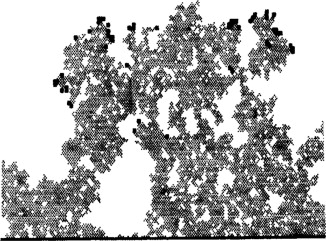
\includegraphics{chapter2/figures/perc1.jpg}
    \caption{A space-time representation of an epidemic spreading at the critical threshold. The spatial (horizontal) and time (vertical) axis show self-similar propagation of diseased individuals in grey, produced by \cite{GRASSBERGER1986273}}
    \label{fig:1d_perc_basis}
\end{figure}

The original formulation of percolation theory was first used to describe properties of a fluid and the bonds which form between molecules \cite{perco_origin} (the reader may jump to \ref{fig:ch3-perc-invariance} for an account of percolation). The problem was posed on a graph\textemdash illustrated in terms of vertices and edges. However re-interpretations were subsequently put forward by physicists studying material sciences, naturally on a lattice. \cite{Essam_1980}. The attractive feature of this new paradigm was that percolation demonstrated a phase-transition. Thus, percolation could be treated with scaling theory used in the study of critical-phenomena. Accordingly, early work rigorously ensued to map out the behaviour of percolation around criticality in terms of critical exponents \cite{STAUFFER19791}. 

Different flavours of percolation models, such as, site or bond percolation were described to model different processes. Percolation proved a convenient theory and various phenomena including, gelation, magnetism and telecommunications were described \cite{trove.nla.gov.au/work/26493727}. Interestingly, forest fires were also applicable to a description within percolation theory \cite{MacKay_1984}. This was a short conceptual jump from time-dependant percolation used to study the growth of crystals \cite{Family_1985}. 

A fire spreading through a population of trees is not to dissimilar to a disease spreading through a population. This lead to a general epidemic-formalisation within percolation-based framework when \cite{pub.1059067807} argued that epidemics were in the same universality class as percolation. It is alluring to remark how modelling the same processes with different microscopic interactions (e.g. different lattice geometries) lead to the macroscopic behaviour should they have the same universality class\textemdash see chapter \ref{fig:ch3-perc-invariance} for more information.

Beginning with a simple $SIR$ framework put forward by \cite{kermack-model}, the field of epidemiology was already well established around the time percolation theory was conceived \cite{baily1975mathematical}. In particular, initial assumptions about population mixing could be relaxed with more elaborate spatial-contact models, naturally, percolation theory could serve as a useful tool when developing spatially-structured epidemic models.

A fractal-like pattern of epidemics was observed by \cite{GRASSBERGER1986273}, shown in Figure \ref{fig:1d_perc_basis}. Parsimoniously describing Figure \ref{fig:1d_perc_basis}, lighter grey sites represent removed individuals, black sites indicate actively infected sites and white sites indicate unaffected sites. All lattice sites in the bottom row were initially infected and the infection can be seen to propagate from the bottom up. The lattice was initialised at the critical-density $p\sim p_c$ culminating in a fractal-like pattern. \cite{GRASSBERGER1986273} did not attribute the hosts of this model to be trees, but instead a general host-population with very low mobility. Local interactions between hosts and infected were elucidated as vast simplifications and long-range interactions (following a power-law) were discussed\textemdash we shall see how these ideas form a important component of modelling tree disease.

The behaviour of percolation-based epidemic models continued (e.g. \cite{pub.1060474189, pub.1059069981}) to be investigated with various methods such as renormalisation-groups and Monte-Carlo, the critical exponents were found along with phase transition graphs characterising epidemic (super-critical) or extinction (sub-critical) regimes. The properties of both epidemics and forest fire percolation models were studied together in \cite{pub.1052857560}, highlighting their similarity.

The first ecological application came in \cite{pub.1031591030} where forest fire (and epidemic) percolation models were adapted in order to study landscape disturbances. Broadly speaking, landscape disturbances constitute a broad array of physical process which lead to a rapid ecological change, this could include invasion of pests, climate-change and fire.

\textemdash\cite{GRASSBERGER1983157} <- reference for early considerations towards percolation as a model for tree diseases and percolation
\textemdash\cite{SANDER2002293}, read and get more info + research links

\section{Early warning signals}

\label{section:ews}
\begin{itemize}
    \item Set the scene for chapters 1 and 2, what are early warning signals and how did they develop ?
    \item Review Siro's paper and give examples of how early warning signals have been used to increase tree-health and resilience 
\end{itemize}


\section{Ash dieback}

% WORK IN PROGRESS
Ash dieback will be the subject of chapter \ref{ch:6} and presents an interesting case-study of an emerging epidemic. Ash dieback is lethal to ash and affects trees of all ages, although age is a significant component of the disease severity \cite{marccais2017estimation}. % this section should relate the biology of ADB to the model, a literature review in ch2 should explore a more complete picture

Ash dieback, caused by the fungus \textit{H.pseudoalbidus} (HP), is a highly seasonal \cite{bengtsson2014seasonal} and follows a complicated, yearly, polycyclic infection cycle. The ADB pathosystem, has been the subject of much research over the years, the taxonomy, symptoms and life-cycle of the pathogen are well-known \cite{https://doi.org/10.1111/mpp.12073}. Although, compartmentalised models of ADB have a noticeable absence in the literature.

The control of ash dieback in an established focus of infestation is virtually impossible, as noted by \cite{havrdova2017environmental}. Moreover, it is already well recognised that ADB will wipe out the vast majority of ash, in Europe and Great Britain alike.

% draw analogy between exponential kernel of \cite{} <- tracking adb and \cite{} <- landscape spread of adb
% commonly referred to as \textit{H.pseudoalbidus}-\textit{F. excelsior}


The controlling ADB in both natural and artificial ash stands is incredibly challenging, verging on impossible if the pathogen is already established \cite{havrdova2017environmental}.

